\documentclass[%fontsize=12pt,
paper=a4,%Papierformat
parskip=half,%Abstand statt Einzug für Absatzwechsel
headsepline,%Linie unter Kopfzeile
plainheadsepline,%Linie unter Kopfzeile bei Kapitelanfängen
twoside=false,%Einseitiger Satz
headings=small%Kleine Kapitelüberschriften
]{scrreprt}

%%%PAKETE	
%%Grundlegende Pakete
\usepackage[utf8]{inputenc}%Eingabezeichensatz
\usepackage[T1]{fontenc}%Verwende Type 1-Schriften
\usepackage{lmodern}%Schriftart
\usepackage[ngerman]{babel}%Deutsche Silbentrennung
\usepackage{microtype}

%% Keine Warnings bei float
\usepackage{scrhack}

%%Pakete für Zeichen
\usepackage{textcomp}%Symbole
\usepackage{latexsym}%Symbole
\usepackage[style=german]{csquotes}%Anführungszeichen mit \enquote{}

%%Pakete für Schriften
\usepackage{color}

%%Pakete für Formatierung
\usepackage{scrpage2}%Paket für KOMA-Script Kopf- und Fußzeilen
\usepackage{geometry}%Seitenränder anpassen

%%Pakete für Tabellen
\usepackage{multirow}
\usepackage{booktabs}

%%Pakete für Mathematik
\usepackage{amsmath}%Mathematikpakte der AMS
\usepackage{amsfonts}%Schriften der AMS
\usepackage{amssymb}%Symbole der AMS
\usepackage{nicefrac} %Schräger Bruch

%%Pakete für Grafiken
\usepackage{graphicx}

%%Pakete für Quelltext
\usepackage{listings}

%%Sonstige Pakete
\usepackage[iso]{datetime}
\usepackage{ifthen}
\usepackage{caption}
\usepackage{subcaption}

%%%BEFEHLE
%%Befehl für typographisch korrekten Abstand bei Abkürzungen wie "z. B." oder "d. h."
\newcommand{\abk}[2]{{#1}.\,{#2}.}

%%Sonstige Befehle und Variablen
\newboolean{draft}

%%%EINSTELLUNGEN
%%Grundlegende Einstellungen für das Dokument
\setboolean{draft}{true}

\title{Laborbericht}
\subtitle{Komplexe Informationstechnische Systeme - Grundlagen}
\author{Lennard Pfennig \and Simon Buttgereit \and Michael Pfeiffer}
\date{TODO DATUM}
\subject{Sommersemester 2016}
\publishers{Version alpha}%raped field

% Wenn Boolean draft gesetzt ist, setze Hinweis auf Titelseite
\ifthenelse{\boolean{draft}}{%if then
	\titlehead{\centering{\textcolor{red}{
		{\Huge Entwurf}\\
		Kompiliert: \today \ \currenttime
	}}}
}{}

%%Schriftart
\renewcommand{\familydefault}{\sfdefault}%Serifenlose Schrift

%%Seitenrandeinstellungen
\geometry{a4paper,left=25mm,right=25mm, top=30mm, bottom=30mm}

%%Anpassungen von Kapitelüberschriften
\renewcommand*{\chapterheadstartvskip}{\vspace{-5mm}}

%%Anpassen von Kopf- Fußzeilen
\pagestyle{scrheadings}
\automark{chapter}
\ohead[\headmark]{\headmark}
\chead{}
% Wenn Boolean draft gesetzt ist, setze Hinweis auf jeder Seite oben links
\ifthenelse{\boolean{draft}}{%if then
	\ihead[\textnormal{\textcolor{red}{Entwurf - Kompiliert: \today \ \currenttime}}]
	{\textnormal{\textcolor{red}{Entwurf - Kompiliert: \today \ \currenttime}}}
}
{%else
	\ihead{}
}

%%Einstellungen für Quelltext
\lstset{ %
language=c++,%Standardsprache
basicstyle=\footnotesize\ttfamily,
breaklines=true,
%showstringspaces=false,
flexiblecolumns=true,
numbers=right,
numberstyle={\tiny}
}

%%Einstellungen für die PDF-Erzeugung
%Hyperref muss als letztes aufgerufen werden!
\usepackage[pdfstartview = FitH,%Seiten auf volle Breite anzeigen
bookmarksopen=true,bookmarksnumbered=true,%Inhaltsverzeichnis im PDF links anzeigen
colorlinks,linkcolor=black,plainpages=false,hypertexnames=false,citecolor=black,filecolor=black,urlcolor=black,%Keine Hervorhebung von Links
pdfpagelabels,pdftitle={Laborbericht},
pdfauthor={Lennard Pfennig, Simon Buttgereit und Michael Pfeiffer},
pdfsubject={Komplexe Informationstechnische Systeme}]{hyperref}%PDF-Informationen

\pdfcompresslevel=0%PDF-Kompression (Bilder)

\begin{document}
\maketitle

\tableofcontents

\chapter{Einleitung}
Dieser Laborbericht dokumentiert das Praktikum \enquote{Kugelfallversuch} zur Vorlesung \enquote{Komplexe Informationstechnische Systeme -- Grundlagen} der Gruppe im Sommersemester 2016.
Der Bericht umfasst (neben dieser Einleitung) drei Kapitel.

\cref{k_analyse} umfasst eine knappe Beschreibung des Versuchsaufbaus, TODO

Im darauffolgenden \cref{k_design} wird das entworfene Softwaresystem in seinem Aufbau und seiner Funktion beschrieben.
Anschließend werden die Grenzwerte, unter denen das System seine Funktion erfüllt, dargestellt und eine Fehlerbetrachtung durchgeführt.

In \cref{k_implementierung} wird schließlich die Implementierung des Systems detailliert und eine Validierung durchgeführt.

\chapter{Analyse}\label{k_analyse}
\section{Versuchsaufbau}\label{s_versuchsaufbau}

Der Versuchsaufbau besteht aus einer drehbaren Scheibe mit Loch und einer Kugelabwurfvorrichtung.
Diese wird mit einem Servomotor bedient (siehe \cref{subs:aktoren}).
Abbildung \ref{img:versuchsaufbau} zeigt eine schematische Darstellung.
Da das Ziel des Praktikums ist, Kugeln durch das Loch fallen zu lassen, ist die Abwurfvorrichtung so angebracht, dass die Kugeln bei einer bestimmten Position der Scheibe durch dieses fallengelassen werden können.
Die Unterseite der Scheibe besitzt zwei Farbschattierungen (hell und dunkel), welche durch einen Photosensor erkannt werden können.
Weiterhin sind zwei Magneten angebracht, welche durch einen Hall-Sensor erkannt werden.
Im Folgenden wird genauer auf die Sensoren eingegangen.

\begin{figure}[h] \centering
	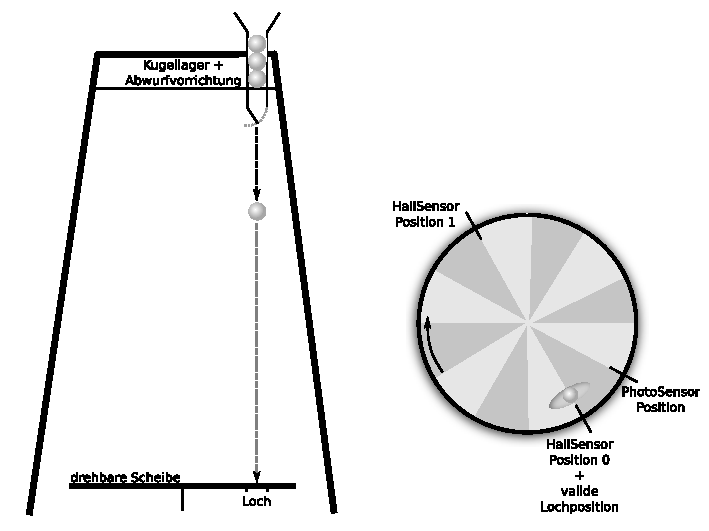
\includegraphics[width=\textwidth]{images/aufbau.pdf}
	\caption{schmatischer Versuchsaufbau - v.\,l.\,n.\,r. Seitenansicht Gesamtaufbau, Drehbare Scheibe}
	\label{img:versuchsaufbau}
\end{figure}

\begin{center}
\begin{tabular}{lc} 
	\textbf{Eigenschaft} 	& \textbf{Beschreibung}	\\
	\toprule
	\multicolumn{2}{c}{Tisch}\\ 
	\midrule
	Abwürfhöhe 	& 750\,mm \\
	Anzahl Schwarze Felder 	& 6 \\
	Anzahl Weiße Felder 	& 6 \\
	Lochlänge innen 	& 55\,mm \\
	\midrule 
	\multicolumn{2}{c}{Kugel}\\ 
	\midrule
	Masse 	& 8.5\,g \\
	Durchmesser 	& 12\,mm \\
	\bottomrule
\end{tabular}
\end{center}

\subsection{Sensoren}
Der Hall-Sensor zeigt zwei mal pro Umdrehung exakt die Position der Scheibe an.
Dies geschieht, wenn das Loch an \texttt{HallSensorPosition1} und \texttt{HallSensorPosition0} ist (siehe Abb. \ref{img:versuchsaufbau}), wobei zweiteres der Position entspricht, an welcher die Kugel durch das Loch fallen muss.
An den Positionen wechselt die Ausgabe der Sensoren auf den entsprechenden Wert, daher 1 bzw. 0.

Der Photosensor gibt abhängig davon, ob er eine helle oder dunkle Fläche vor sich hat eine 1 oder 0 aus.
Da die Felder auf der Unterseite der Scheibe gleichmäßig verteilt sind (siehe Abb. \ref{img:versuchsaufbau}), kann er nicht zur Positionsbestimmung, jedoch für die Bestimmung der Drehgeschwindigkeit verwendet werden.

Die Sensorwerte für Hall- und Photosensor einer Scheibenumdrehung sind in Abb. \ref{img:sensorwerte} dargestellt.

Der dritte Sensor ist ein Trigger, welcher 1 ausgibt, wenn er gedrückt wird.
Dieser soll dafür benutzt werden den Kugelfall zu initiieren, bzw. die Anzahl der Kugeln zu bestimmen, welche zum nächstmöglichen Zeitpunkt fallen gelassen werden sollen.

Weiterhin gibt es einen Dreiwegeschalter (Switch) und zwei Buttons, welche nicht benutzt werden.

\subsection{Aktoren}
\label{subs:aktoren}
Wie bereits beschrieben, wird die Abwurfvorrichtung durch einen Servo gesteuert.
Sobald sich dieser aus seiner Ursprungsposition auf einen Winkel von 30° dreht, fällt eine Kugel aus dem Magazin und die nächste Kugel wird automatisch nachgeladen.

Weiterhin gibt es noch einige LEDs, welche in der Implementierung keine besondere Rolle besitzen.

\subsection{Ansteuerung der Komponenten}
Für das Auslesen der Sensoren und die Ansteuerung der Aktoren stehen ein Arduino UNO und eine Art Blackbox zur Verfügung.
Zweitere sorgt dafür, dass die Sensoren und Aktoren direkt an die Pins des Arduino angeschlossen sind, und einfach mittels \texttt{digitalWrite} und \texttt{digitalRead} angesteuert werden können.
Die Belegung der Pins sind in der folgenden Tabelle beschrieben:

\begin{center}
\begin{tabular}{cll} 
	\textbf{Pin} 	& \textbf{In/Out} & \textbf{Funktion}	\\
	\toprule
	2 &	Input &	Photosensor \\
	3 &	Input &	Hallsensor\\
	4 &	Input &	Trigger\\
	5 &	Input &	Switch\\
	7 &	Output &	Blackbox LED gelb\\
	9 &	Output &	Servo\\
	10 &	Input &	Button 1\\
	11 &	Input &	Button 2\\
	12 &	Output &	LED 1\\
	13 &	Output &	LED 2\\
	\bottomrule
\end{tabular}
\end{center}

\begin{figure}[h] \centering
	\includegraphics[width=\textwidth]{images/generated/sensor_messwerte1.pdf}
	\caption{Sensorzyklus einer Scheibenumdrehung}
	\label{img:sensorwerte}
\end{figure}

\section{Fallzeit der Kugel}\label{analyse_fallzeit}
Um die Fallzeit einer Kugel zu berechnen wird die Formel für den freien Fall im homogenen Feld
\begin{align}
	t(h) = \sqrt{\frac{2h}{g}}
\end{align}
verwendet.
Setzt man die oben beschriebenen (am Versuchsaufbau gemessenen) Werte ein
\begin{align}
t(h) &= \sqrt{\frac{2 \cdot 0.75m}{9.81\,\nicefrac{m}{s^2}}} \\
	 &= 0.391\,s \\
	 &= 391\,ms
\end{align}
so erhält man eine eine Fallzeit von 391\,ms für eine Kugel.

\subsection{Drehbewegung der Scheibe}
\label{subs:dreh_approx}
Der Aufbau der Scheibe wurde bereits beschrieben.
Für eine korrekte Berechnung der Abwurfzeit wird des weiteren eine Beschreibung des Drehverhaltens benötigt.
Bei Messungen konnte folgendes Polynom für die Drehgeschwindigkeit [U/min] über der Zeit [s] (siehe Abb. \ref{img:drehgeschw}) festgestellt werden:
\begin{align}
	f(t) = 151.16 - 1.57 \cdot t + 0.0037 \cdot t^2 \label{form:f(t)}
\end{align}
Umgerechnet in die Funktion für die Zeit [ms] pro Umdrehung ergibt sich:
\begin{align}
	h(t) 	&= \frac{60000}{151.16 - 1.57t + 0.0037 \cdot t^2} \\
	    	&= \frac{1.62162\cdot 10^7}{(t-276.65) (t-147.674)} \label{form:h(t)}
\end{align}
Die Umkehrfunktion, daher die Funktion, um mittels der Zeit pro Umdrehung die Position auf $h(t)$ zu berechnen, lautet:
\begin{align}
	h^{-1}(t) 	= 212.162 \pm \frac{0.27027 \cdot \sqrt{56933\cdot t^2 + 2.22\cdot 10^8 \cdot t}}{t} \label{form:h-1(t)}
\end{align}
wobei für die Berechnungen nur die Subtraktion benötigt wird:
\begin{align}
	h^{-1}_{real}(t) 	= 212.162 - \frac{0.27027 \cdot \sqrt{56933\cdot t^2 + 2.22\cdot 10^8 \cdot t}}{t} \label{form:h-1(t)_2}
\end{align}
Da später die Bremsgeschwindigkeit bzw. die Beschleunigung und damit Anstieg der Zeit pro Umdrehung vorausgesagt werden soll, muss die erste Ableitung von $h(t)$ berechnet werden:
\begin{align}
	h'(t) 	= \frac{6.88093\cdot 10^9 - 3.24324 \cdot 10^7 \cdot t}{(t^2 - 424.324\cdot t + 40854.1)^2} \label{form:h'(t)}
\end{align}

% Approximationskurve
\begin{figure}[hb] \centering
	\includegraphics[width=\textwidth]{images/generated/Data2.pdf}
	\caption{Drehgeschwindigkeit über der Zeit approximiert mit der Funktion $f(t)$ (siehe Formel \ref{form:f(t)})}
	\label{img:drehgeschw}
\end{figure}


\chapter{Design}

% Systemüberblick (3 Komponenten)

% Vorgehen

% Grenzwerte

% Fehlerbetrachtung
\chapter{Implementierung}\label{k_implementierung}
\section{Übersicht über die Klassenhierarchie}
Die in \cref{design_systemueberlick} vorgestellten Komponenten werden durch eine Klassenhierarchie implementiert.
Eine Gesamtübersicht der Klassenhierarchie gibt \cref{uml:class_diagram}.
Im Folgenden werden nun die einzelnen Gruppen genauer betrachtet.
Im Quellcode liegen Klassen derselben Gruppe im gleichen Ordner.

\subsection{Hardware}
Die abstrakte Basisklasse dieser Gruppe ist die \identifier{Component}.
Über sie wird lediglich die entsprechende Pin-Nummer der Komponente zugeordnet.
Von \identifier{Component} erben drei Klassen: \identifier{LED}, \identifier{Sensor} sowie \identifier{Release}:

\begin{itemize}
	\item Die abstrakte Basisklasse \identifier{LED} stellt Methode zum Ein-, Aus- und Umschalten von LEDs bereit.
In den konkreten abgeleiteten Klassen (wie \identifier{GreenLED}) erfolgt dann lediglich noch die Zuordnung zum korrekten PIN.
	\item Bei \identifier{Sensor} handelt es sich ebenfalls um eine abstrakte Basisklasse, die das Abfragen von Sensoren erlaubt.
Ähnlich wie bei den LEDs wird dann in den abgeleiteten Klassen \identifier{PhotoSensor}, \identifier{HallSensor} und \identifier{Trigger} nur noch die PIN-Nummer korrekt gesetzt.
	\item Die konkrete Klasse \identifier{Release} kapselt die konkrete Ansteuerung des Servomotors, und stellt diese über die Methoden \identifier{open()} und \identifier{close()} zur Verfügung.
\end{itemize}

\begin{figure}[hb] \centering
	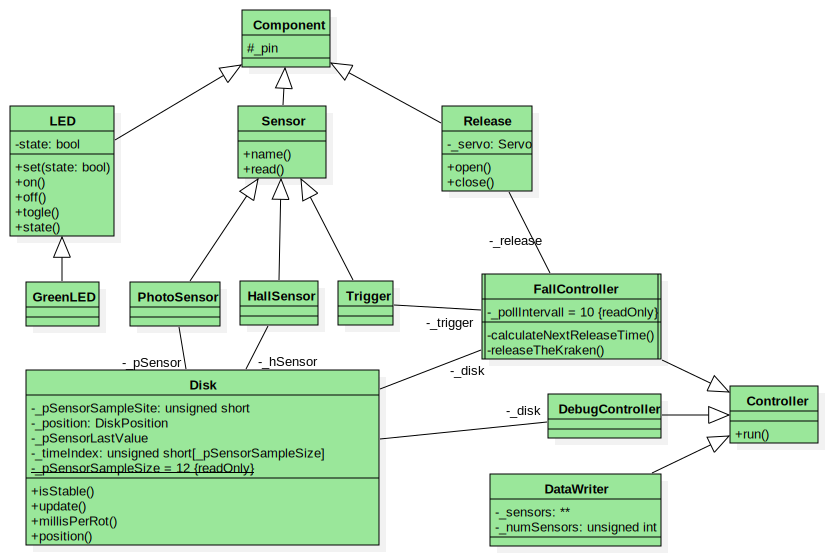
\includegraphics[width=\textwidth]{UML/class_diagram.pdf}
	\caption{Klassendiagramm der Implementierung}
	\label{uml:class_diagram}
\end{figure}

% Kontrollfluss
\begin{figure}[hb] \centering
	\begin{subfigure}[b]{0.4\textwidth}
		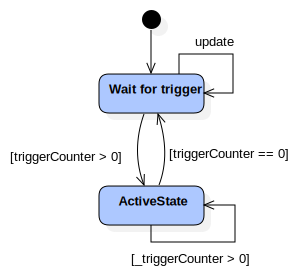
\includegraphics[width=\textwidth]{UML/fallcontroller_simple_loop_statechart.pdf}
		\caption{Einfache Darstellung}
		\label{uml:statechart_simleloop}
	\end{subfigure}\hspace{1cm}
	\begin{subfigure}[b]{0.4\textwidth}
 		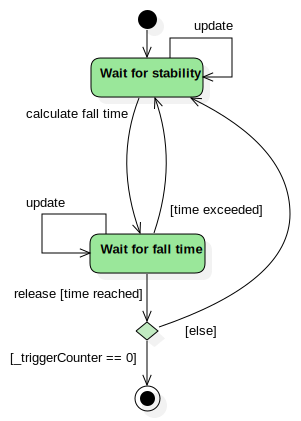
\includegraphics[width=\textwidth]{UML/fallcontroller_active_state_statechart.pdf}
		\caption{Genauere Beschreibung des ActiveStates aus \ref{uml:statechart_simleloop}}
		\label{uml:statechart_activeState}
	\end{subfigure}
	\caption{Beschreibung der Hauptschleife als Zustandsübergangsdiagramm}
	\label{uml:statechart}
\end{figure}

\begin{figure}[hb] \centering
\end{figure}

\begin{figure}[hb] \centering
	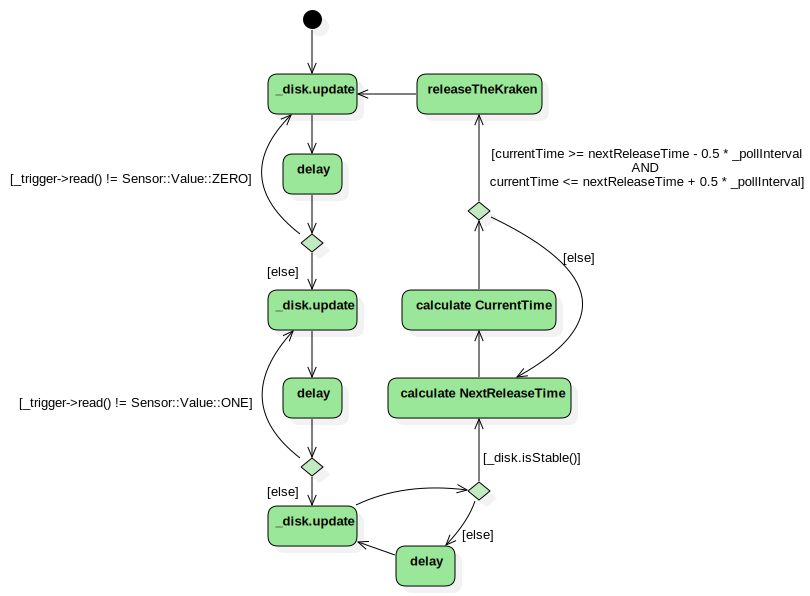
\includegraphics[width=\textwidth]{UML/fallcontroller_loop_activity_diagram.pdf}
	\caption{Genauere Beschreibung der Hauptschleife als Aktivitätsdiagramm}
	\label{uml:activity_diagram}
\end{figure}


% Validierung

%%%%


\end{document}
